\iffalse

\bibliography{..\\bib\\tex.bib}

\fi

\chapter{针对多义词的语义强化模型及相关实验}

多义词是指同一个词语往往会在不同的语言环境下表达出不同的意义,如词语bank既可以表示银行的意思,也可以表示河岸,在这种情况下,如果我们使用传统的词向量嵌入模型进行词向量的学习,则需要用一个词向量表达多个意思,即忽略了一个词语多个不同的意义之间的区别。

在\citep{bengio2006neural}提出了这个问题后,如我们在\ref{sec:intro_poly}中介绍的,\citep{huang2012improving}通过使用K-Means聚类方法对词语的上下文进行聚类的方式,对一个词语的多个不同意义进行区分后再进行词向量的学习。但是,这个方法需要对多义词的语义数量进行预先指定,即假设每个词语都具有某个固定数目的不同意义。这样的处理方法虽然简化了计算与模型设计,但是同时也使得计算出的词向量可能出现冗余,例如,假设将多义词的不同语义的数量指定为10,则对于一个即使没有多个不同意义的词语,这个模型也会生成10个不同的词向量来表示他的语义。下面,我们对这一方法进行进一步的改进,使得改进后的模型可以对不同的词语产生数量不同的词向量。

原有的方法无法动态地指定词向量的数目的主要原因是他使用了K-Means算法来对上下文进行聚类,而K-Means的聚类算法,是需要指定类的个数的。这个限制使得原有的模型必须要预先对语义数目进行指定。在我们的方法中,我们将K-Means聚类算法替换为层次聚类(Hierarchical Clustering)\cite{johnson1967hierarchical}的方式,这个聚类算法不需要显示地指定类别的个数,而是可以通过其他参数来对聚类所得到的类簇数目进行控制。下面我们先对层次聚类进行简单的介绍,再来详细说明我们改进后的算法。

\section{层次聚类}

\begin{figure}
\centering
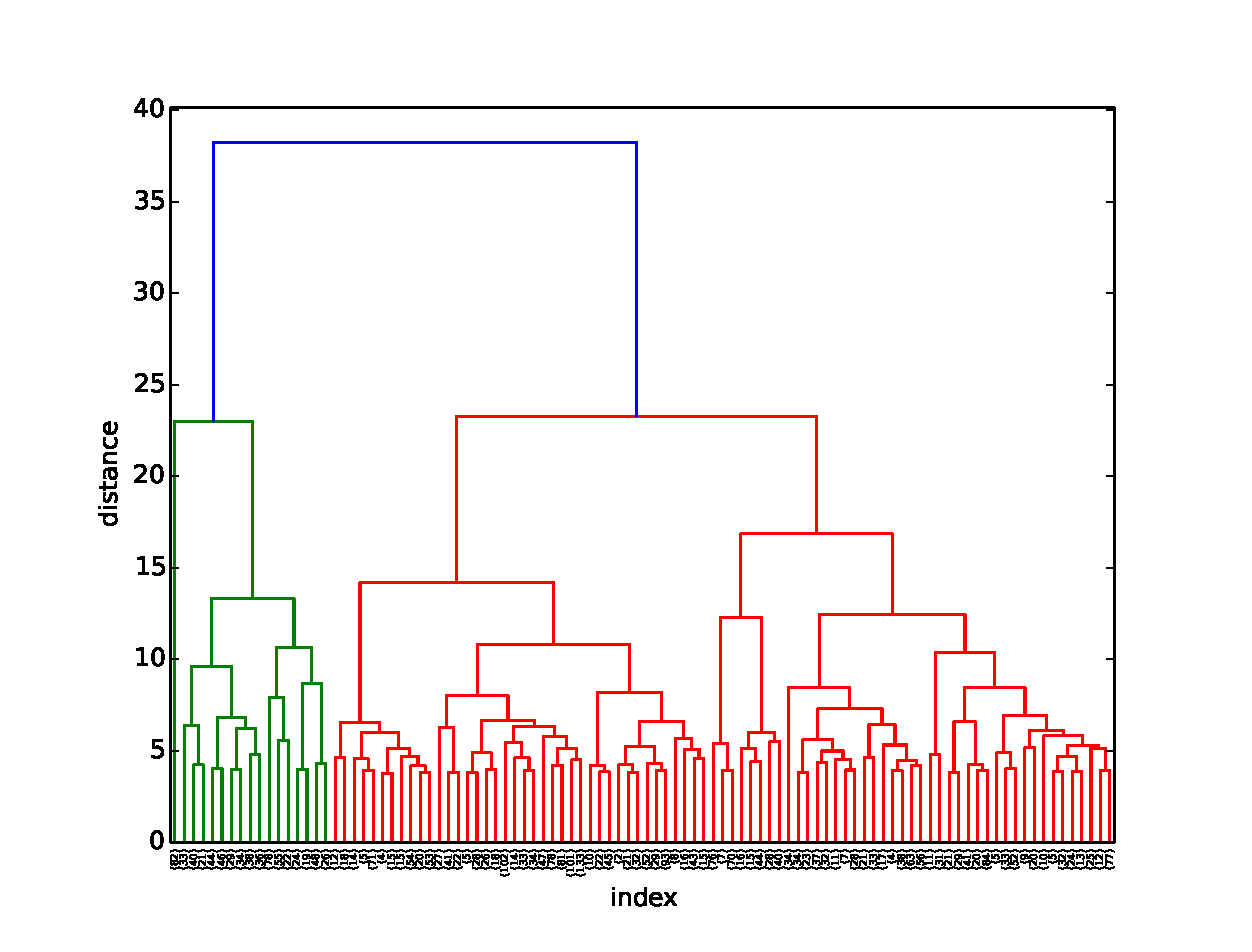
\includegraphics[width=13cm]{hs}
\caption{层次聚类示意图}
\label{fig:hs}
\end{figure}

层次聚类是一种聚类方法,这种方法通过建立树状体系的类簇结构来进行聚类。如图\ref{fig:hs}所示,层次聚类最后得到的结果也不是单独的类簇标号,而是一棵表示类簇结构的树。这种做法的好处在于不需要在聚类的时候对类簇的个数进行限定,在获得这样一棵树之后,在树的任意高度进行分割,就可以获得最后的聚类结果。例如,在图\ref{fig:hs}中高度为30处进行分割,将会得到两个类簇,即左边以绿色标注的类簇,以及右边以红色标注的类簇。

一般来说,层次聚类分为两种,一种是自底向上,另一种是自顶向下。其中,自底向上的算法在最开始将每一个点都视为一个独立的类簇,然后迭代得将两个距离最近的类簇合并为一个类簇,直到只剩下一个类簇,同时,这个逐次合并的过程就会被作为层次聚类所得到的树形结构记录。类似地,自顶向下的方法是在最开始将左右的点都视为同一个类簇,然后通过迭代每次将一个类簇划分为两个类簇,并将这个逐次划分的过程进行记录。

\section{使用层次聚类方法学习多义词对应词向量的算法}

根据\emph{The Distributional Hypothesis},我们知道,当一个多义词以不同的词义出现时,他的上下文应该有所不同。基于这一点,我们可以先对一个词的上下文进行计算并记录,然后再对这些上下文进行聚类,并按照聚类的结果对多义词的语义进行区分。在区分出多义词的多个语义后,我们可以将一个词语的不同语义当成不同词语,然后使用传统的词向量嵌入算法进行词向量的学习。下面我们按照顺序进行介绍。

\subsection{对词语上下文的计算}

一个词语出现的上下文可以被直观描述为词语周边的其他词语的集合,在这里,类似于\citep{huang2012improving},我们将这些词语的加权和作为一个词语的上下文。即先使用\emph{word2vec}工具包计算出词向量,然后对于每个词语,对他周围词语的词向量进行加权求和,并将求和后的向量作为这个词语这一次出现的上下文,即对于语料中的一个词语序列:$w_{i-n}, \cdots,w_{i}, \cdots, w_{i+n}$,词语$w_i$这次出现的上下文为:$\sum_{j \in [-n, n]} \vvec_{i+j} \cdot a_{i+j}$,其中$a_{i+j}$为权值,并满足$\sum_{j \in [-n, n]} a_{i+j} = 1$。为了得到更准确的计算结果,我们将没有什么实际含义的功能词(stop words),例如the, on等,对应的权重设为0。然后我们将Inverse document frequency(IDF)值($w$为某个单词,$d$为某篇文档):
\begin{equation*}
\mathrm{IDF}(w, D) = \mathrm{log} \frac{N}{|\{d | w \in d, d \in D\}| + 1}
\end{equation*}
进行归一化后,作为剩余词的权值:
\begin{equation*}
a_{i+k} = \frac{\mathrm{IDF}(w_{i+k}, D)}{\sum_{j \in [-n, n]} \mathrm{IDF}(w_{i+j}, D)}
\end{equation*}

\subsection{对上下文使用层次聚类分辨多义词的不同语义}

\begin{longtable}{lccc}
% 首页表头
\caption[在三种不同的设定下层次聚类所得到的类簇个数]{在三种设定下对表示上下文的向量进行层次聚类后得到的类簇个数}
\label{tab:num4hc} \\
\toprule[1.5pt]
词语 & 类簇个数(设定一) & 类簇个数(设定二) & 类簇个数(设定三) \\
\midrule[1pt]
country	&	5	&	& \\
pear	&	1	&	3	& \\
cell	&	5	&	312	& \\
light	&	11	&	& \\
play	&	15	&	& \\
mark	&	3	&	& \\
fall	&	4	&	& \\
head	&	5	&	& \\
close	&	12	&	& \\
\endfirsthead
\end{longtable}

在完成表示词语上下文的计算后,我们通过层次聚类算法来对每个词语的不同意思进行区分。在使用层次聚类时,我们使用了Ward Distance\cite{ward1963hierarchical}作为距离计算的方法。同时,为了使不同的词语具有多样且合理的语义数量,我们选择使用Inconsistency作为划分类簇结果的标准。

下面我们将我们使用的层次聚类常的设定与其他两种设定进行对比,通过实验结果来验证说明我们使用的层次聚类的设定的合理性。我们将我们所使用的设定记为设定一,将对比的两种设定分别记为设定二和设定三。其中,设定二使用一个类簇中的最大距离的上限作为划分类簇的标准,设定三使用。如\ref{tab:num4hc}所示,设定一,
通过与其他设定进行比较,我们对层次聚类的设定使得聚类结果的类簇个数具有较好的多样性与合理性。

\subsection{完成多义词的不同语义辨别后得到的词向量}

\begin{longtable}{cc}
% 首页表头
\caption[与多义词不同语义对应词向量距离最近的词语]{对表示上下文的向量进行层次聚类后得到的类簇个数统计表}
\label{tab:near4demo} \\
\toprule[1.5pt]
词语 & 与该词语最近的五个词语 \\
\midrule[1pt]
fall\_1	& autumn, spring, demise, summer\\
fall\_2 	& falling, disappear, erupt, fade, rebound\\
mark\_1	& 400th, 300th, 500th, fiftieth, 200th\\
mark\_2	& signifying, signify, zodiac, syllable, auspicious\\
country\_1	&	nation, Africa, commonwealth, zoo, comoros\\
country\_2	&	reggae, bluegrass, funk, hip-hop, blues\\
\endfirsthead
\end{longtable}

在通过层次聚类,完成对多义词的不同语义进行判别后,我们现在将一个词的不同语义作为不同词语对待,并通过\emph{word2vec}工具重新学习了词向量。

下面那我们通过实验来说明我们获得的词向量可以对多义词的不同词义进行表示与区分。由于词向量携带部分语义信息,我们选择通过罗列与词向量最近的其他词向量所对应的词语,来展示词向量的所携带的语义信息的种类。我们选择了三个多义词,country,fall,mark的部分词向量进行实验,如表\ref{tab:near4demo}所示,我们可以观察到fall所对应的主要的两个语义,落下与季节,被很好得区分开来,country所对应的国家与音乐种类这两个意义也被很好得区分开来,类似地,mark的语义也在他的两个词向量中得到了区分。这说明我们学习获得的词向量确实可以对多义词的不同语义进行较好地区分与表示。